% Replacement text for the current Methods, Results, and Discussion sections.
% Preamble requirement: add \usepackage{booktabs} to main.tex.
% The figure files named below are present in the analysis repository but must
% be copied into the LaTeX project before compilation.

\section{Methods}
\label{sec:methods}

\subsection{Study design}
\label{sec:study_design}

This study assessed the sensitivity of fitted non-stationary temporal ETAS
inference to declustering-derived initial values for the background-rate
function. It was designed as a controlled initialisation experiment rather
than as a comparison of three reduced earthquake catalogues. A single
magnitude-thresholded catalogue, likelihood, background spline, penalty,
triggering-history rule, parameter bounds, optimiser, and set of triggering
parameter starting values were used throughout the main experiment. The only
quantity varied between the three main fits was the initial background-rate
function constructed from Gardner--Knopoff, nearest-neighbour, or
Reasenberg-style declustering.

The analysis followed four linked stages. First, exploratory analysis and
magnitude-completeness diagnostics were used to define a common analytical
catalogue. Second, three structurally different declustering schemes were
applied to that catalogue and their event-level classifications were
compared. Third, the resulting background-like events were converted into
three smooth background-rate starting functions. Finally, the same
non-stationary ETAS model was fitted from each starting function, and the
initial and final between-method differences were compared. A limited
model-specification analysis examined spline flexibility and the length of
the triggering history while holding the nearest-neighbour initialisation
fixed.

\subsection{Earthquake catalogue and preprocessing}
\label{sec:data_preprocessing}

The supplied catalogue was obtained through the Southern California
Earthquake Data Center (SCEDC) SCSN catalogue-search interface
\citep{scedc2013,scedc_catalog_search2026}. The file covers 20 May 2000 to 20
May 2026 and contains origin date and time, event and geographic type,
magnitude and magnitude type, epicentral latitude and longitude, focal depth,
a quality field, event identifier, and two phase-related count fields. The
downloaded file contained 167,584 records. All records were labelled as local
earthquakes, and event identifiers were unique.

The observed, rather than requested, ranges in the supplied file were
$-0.98$ to $7.10$ for magnitude, $34.500^\circ$ to $36.500^\circ$ N for
latitude, $118.99983^\circ$ to $116.00400^\circ$ W for longitude, and
$-2.3$ to $28.9$ km for depth. These observed ranges should not be interpreted
as the original catalogue-query limits.
% [需要作者确认：SCEDC 查询时实际设置的经纬度、深度和震级上下限，以及文件下载日期。]

Origin date and time were combined into a timestamp; magnitude, latitude,
longitude, and depth were converted to numeric variables; and events were
sorted chronologically. Rows missing any of these required variables would
have been removed. The supplied file contained 167,584 parseable records and
the preprocessing step retained the same number, so no record was excluded by
this missing-value rule. No event was removed solely because it shared an
origin timestamp with another event; distinct event identifiers were treated
as distinct catalogue records.

Exploratory data analysis was performed before selecting a completeness
threshold. Annual and monthly event counts and the cumulative event count
were used to identify temporal changes in recorded activity. Daily counts in
a 30-day window around the catalogue's largest event were used to describe
short-term concentration, and epicentral maps were used to assess the
geographical coverage of the data and to contrast 2019 with the rest of the
observation period. These analyses were descriptive; their purpose was to
identify catalogue features requiring explicit treatment in the subsequent
completeness and sensitivity analyses.

\subsection{Magnitude completeness}
\label{sec:magnitude_completeness}

The magnitude of completeness, $M_c$, is the threshold above which the
catalogue is treated as sufficiently complete for the intended analysis.
Events below $M_c$ can be preferentially missed when monitoring performance
changes or when an intense sequence temporarily reduces the detectability of
small events. Such omissions can affect estimated clustering patterns and
ETAS parameters, so completeness was assessed before constructing the common
analytical catalogue.

The primary estimator was the Woessner--Wiemer $b$-value stability method
(MBS-WW), selected because comparative work has found that the performance of
catalogue-based $M_c$ estimators varies under heterogeneous completeness and
because MBS-WW provides a stability-based diagnostic rather than relying only
on the modal magnitude \citep{wang2025magnitude}. The method uses the
Gutenberg--Richter relationship
\[
\log_{10}N(M)=a-bM,
\]
where $N(M)$ is the number of events with magnitude at least $M$. For a
candidate threshold $m$, the $b$-value was estimated by
\[
\hat b(m)=\frac{\log_{10}(e)}
{\bar M_m-(m-\Delta M/2)},
\]
where $\bar M_m$ is the mean magnitude among events with $M\geq m$ and
$\Delta M=0.1$. Candidate thresholds were considered in increments of 0.1.
MBS-WW selected the lowest candidate at which the estimated $b$-value was
within its estimated uncertainty of the mean $b$-value over the next 0.5
magnitude units.

The MBS-WW candidate was checked using a Gutenberg--Richter goodness-of-fit
statistic (GFT), which measures agreement between the observed and fitted
cumulative frequency--magnitude distributions. A 95\% fit was considered
first and a 90\% fit was used as a secondary diagnostic
\citep{wang2025magnitude,pavlenko2022comparative}. The GFT was used to assess
the MBS-WW candidate, not as an independent estimator that automatically
replaced it.

The exploratory analysis identified 2019 as an unusually active period.
MBS-WW was therefore repeated for 2019 and for all other years combined.
Shorter-term variation was assessed in chronologically ordered windows of
1,000 successive events, advanced by 250 events. The MBS-WW estimate and
the $b$-value at thresholds 1.7 and 2.0 were recorded for each window. A
single operational threshold was then chosen for all subsequent comparisons,
so that the three declustering methods and all main ETAS fits used identical
events. This common threshold was a design compromise between retaining
events and reducing temporal heterogeneity; it was not interpreted as proof
that every part of the catalogue, especially 2019, was strictly complete
above that value.

\subsection{Assessment of triggering and background non-stationarity}
\label{sec:nonstationarity_screening}

Two preliminary comparisons were used to motivate the final temporal ETAS
specification. First, a homogeneous Poisson process with one constant rate
parameter was compared with a stationary temporal ETAS model containing a
constant background rate and four triggering parameters. Second, the
stationary ETAS model was compared with a diagnostic non-stationary model in
which the background rate was piecewise constant over approximately five-year
intervals while the triggering parameters were common across intervals. With
the 26-year observation period, this produced six background intervals and
ten fitted parameters in total. These models used the complete $M\geq2.0$
catalogue and the available within-catalogue triggering history.

Models were compared using maximised log-likelihood, Akaike information
criterion (AIC), and Bayesian information criterion (BIC). The piecewise
model was used only to assess whether relaxing a constant-background
assumption improved relative fit; it was not the final background model.
These comparisons showed whether allowing the background rate to change over
time fitted the data better than assuming a constant background rate. They
only compared alternative models, however, and did not test whether the final
spline-based model adequately described the observed event times; that would
require separate residual diagnostics.

\subsection{Declustering methods}
\label{sec:declustering}

\subsubsection{Common comparison framework}

Three methods with contrasting structural assumptions were applied to the
same $M\geq2.0$ catalogue: the Gardner--Knopoff window method
\citep{gardner1974}, a deterministic nearest-neighbour cluster construction
based on the space--time--magnitude framework of \citet{zaliapin2013} and
\citet{zaliapin2020declustering}, and a Reasenberg-style interaction method
\citep{reasenberg1985}. One pre-specified baseline configuration was used for
each method. The settings were not selected to maximise agreement between
methods or to improve the subsequent ETAS fits.

The method-specific outputs were reduced to a common indicator,
\[
B_i^{(d)}=
\begin{cases}
1, & \text{event $i$ is background or the mainshock of a cluster under method $d$},\\
0, & \text{event $i$ is a foreshock or aftershock under method $d$},
\end{cases}
\]
where $d\in\{\mathrm{GK},\mathrm{NN},\mathrm{R}\}$. The term
``background-like'' is used for $B_i^{(d)}=1$ because these classifications
are algorithmic labels, not observed ground truth.

\subsubsection{Gardner--Knopoff window method}

The Gardner--Knopoff method assigns magnitude-dependent spatial and temporal
windows \citep{gardner1974,vanstiphout2012}. The implemented spatial window
was
\[
D(M)=10^{0.1238M+0.983}\ \mathrm{km},
\]
and the temporal window was
\[
T(M)=
\begin{cases}
10^{0.5409M-0.547}\ \mathrm{days}, & M<6.5,\\
10^{0.032M+2.7389}\ \mathrm{days}, & M\geq6.5.
\end{cases}
\]
Events were processed from larger to smaller magnitude, with earlier events
processed first in the event of a tie. An unassigned event was treated as a
potential mainshock, and currently unassigned events inside its spatial and
temporal windows were assigned to its cluster. Cluster members before the
mainshock were labelled foreshocks and later members were labelled
aftershocks. Unclustered events were labelled background. The baseline used
the full pre-mainshock temporal window, corresponding to a temporal-window
proportion of 1.0.

\subsubsection{Nearest-neighbour method}

For event $i$, each earlier event $j$ was evaluated using
\[
\log_{10}\eta_{ij}
=\log_{10}t_{ij}
+d_f\log_{10}r_{ij}
-b(M_j-M_c),
\]
where $t_{ij}$ is elapsed time in years, $r_{ij}$ is epicentral distance in
kilometres, $M_j$ is the earlier event's magnitude, and $b$ is the
Gutenberg--Richter estimate from the common catalogue. The analysis used
$d_f=1.6$, $M_c=2.0$, and $\hat b=0.8152$. A value of $d_f$ between 1 and 2
is consistent with the range commonly used for epicentral locations, although
the published stochastic declustering algorithm recommends estimating it for
the catalogue where possible \citep{zaliapin2020declustering}.

The earlier event with minimum $\eta_{ij}$ was assigned as the potential
parent. A two-component Gaussian mixture was fitted to the finite
$\log_{10}\eta_i$ values using a fixed random seed of 123. The fitted
unequal-variance model had component means $-5.120$ and $-1.432$; the
posterior-equality rule gave a threshold of $-2.740$. Parent--child links
below this threshold were retained and converted into connected components.
The largest event in each component was labelled the mainshock, with earlier
and later members labelled foreshocks and aftershocks, respectively.
Singletons were labelled background.

This construction uses the nearest-neighbour proximity and its bimodal
distribution, but it is not the stochastic, spatially adaptive thinning
algorithm proposed by \citet{zaliapin2020declustering}. It is therefore
described as a deterministic nearest-neighbour cluster classification for the
present sensitivity experiment.

\subsubsection{Reasenberg-style interaction method}

The Reasenberg-style procedure processed events chronologically and allowed
clusters to grow or merge when a new event satisfied temporal and spatial
interaction criteria for an existing member. Candidate parents were limited
to events within the preceding $\tau_{\max}=10$ days. The temporal look-ahead
was bounded between $\tau_{\min}=1$ and $\tau_{\max}=10$ days and depended on
the maximum magnitude and elapsed duration of the evolving cluster. Spatial
interaction was based on a magnitude-dependent radius obtained by multiplying
$10^{0.4M-1.2}$ km by $r_{\mathrm{fact}}=10$.

The baseline settings were $\tau_{\min}=1$ day, $\tau_{\max}=10$ days,
$p_1=0.95$, $x_k=0.5$, $x_{\mathrm{meff}}=4.0$, and
$r_{\mathrm{fact}}=10$. Groups linked directly or indirectly were merged.
The largest event in each multi-event group was labelled the mainshock, and
other members were labelled by whether they occurred before or after it.
The term Reasenberg-style is retained because the implementation reproduces
the broad adaptive interaction and cluster-merging ideas, but not every step
of the original \texttt{CLUSTER2000} implementation.

\subsection{Comparison of declustering outputs and construction of ETAS starts}
\label{sec:declustering_comparison}

For each method, the number and proportion of background-like events were
recorded. Pairwise raw agreement summarised agreement over both classes;
Jaccard similarity measured overlap between the two background-like sets; and
Cohen's $\kappa$ measured agreement beyond chance. The proportion of events
without a unanimous three-method classification was also calculated. Because
background-like events were rare during 2019, the same summaries were
repeated for 2019 and non-2019 events to distinguish high raw agreement caused
by class imbalance from agreement on the minority background-like class.

For method $d$, background-like events were aggregated by calendar month to
give a rate $r_d(m)$ in events per day. Pairwise mean absolute error (MAE),
root mean squared error (RMSE), and Pearson correlation were computed for the
raw monthly series, both over the full period and within 2019. These measures
are descriptive effect-size summaries; no independence assumption, formal
null hypothesis, or $P$-value was attached to them.

For declustering method $d$ and calendar month $m$, let $n_{dm}$ denote the
number of events classified as background-like and let $E_m$ denote the
number of days for which that month lay inside the ETAS observation interval.
The observation interval was defined by the first and last retained
$M\geq2.0$ events. Consequently, $E_m$ was the full number of days for an
interior month but only the observed part of the month at the beginning and
end of the catalogue. Using $E_m$ avoided treating these two partial months
as if they had been observed for a complete calendar month.

The monthly value used to construct the starting background was
\[
y_{dm}=\log\left(\frac{n_{dm}+0.1}{E_m}\right).
\]
The logarithm was used because the final ETAS model represents the background
as $\log\mu(t)=B(t)\boldsymbol\beta$; fitting the starting values on the same
scale ensures that $\mu(t)=\exp\{B(t)\boldsymbol\beta\}$ is positive. Some
months contained no background-like events, for which the unadjusted rate was
zero and its logarithm was undefined. The small fixed pseudo-count of 0.1
made every starting rate finite. It was a numerical device for constructing
initial values, not an additional observed event.

The ETAS optimiser required a vector of spline coefficients rather than a
separate rate for every month. The monthly log rates were therefore projected
onto the same natural-cubic-spline basis used by the final model. With $t_m$
denoting the midpoint of the observed portion of month $m$, the initial
coefficient vector was obtained as
\[
\boldsymbol\beta_d^{(0)}=
\arg\min_{\boldsymbol\beta}
\left\{
\sum_m\left[y_{dm}-B(t_m)\boldsymbol\beta\right]^2
+10^{-4}\lVert\boldsymbol\beta\rVert_2^2
\right\}.
\]
This least-squares projection converted the monthly summaries into a smooth
starting function $\mu_d^{(0)}(t)=\exp\{B(t)\boldsymbol\beta_d^{(0)}\}$ in the
same parameterisation as the fitted background. It was not used to estimate a
separate scientific relationship. The small ridge term stabilised the matrix
calculation if columns of the spline basis were nearly dependent. Both the
pseudo-count and ridge term affected only the starting values; they did not
alter the catalogue or the ETAS likelihood.

For a like-for-like propagation comparison, the three smooth starting
functions were evaluated on the same daily grid as the final fitted
background functions. MAE, RMSE, and correlation were then calculated on this
common grid. This same-grid comparison replaces an earlier diagnostic that
used unweighted monthly rates in the denominator and daily fitted rates in
the numerator.

Declustering was used only to construct these alternative starting
background functions. No event labelled as a foreshock or aftershock was
removed: all three ETAS fits used the same full $M\geq2.0$ catalogue and the
same likelihood specification, so only the starting background function
differed. This controlled design isolated whether differences between the
declustering-derived starts persisted in the fitted ETAS inference.

\subsection{Non-stationary temporal ETAS model}
\label{sec:etas_model}

For event times $t_i$ and magnitudes $M_i\geq M_c$, the fitted temporal ETAS
conditional intensity was
\begin{equation}
\lambda(t_i)=\mu(t_i)+
\sum_{j<i:\,0<t_i-t_j\leq H}
K\exp\{\alpha(M_j-M_c)\}(t_i-t_j+c)^{-p},
\label{eq:etas_intensity}
\end{equation}
where $\mu(t)$ is the background rate in events per day, $K$ is triggering
productivity, $\alpha$ controls its magnitude dependence, $c$ regulates the
short-lag behaviour, $p$ is the temporal decay exponent, and $H$ is the
triggering-history cutoff \citep{ogata1988statistical}. This was a temporal
model: locations and depths informed declustering but did not enter the ETAS
likelihood.

The main analysis used $H=3,650$ days. Events before the start of the supplied
catalogue were unavailable, so only earlier events observed within the
catalogue contributed to triggering. The cutoff is a modelling and
computational approximation, not a claim that older events have no physical
effect.

The time-varying background was represented by
\begin{equation}
\log\mu(t)=B(t)\boldsymbol\beta,
\label{eq:background_spline}
\end{equation}
where $B(t)$ is a natural cubic spline with eight degrees of freedom,
including an intercept and boundary knots at the first and last event times.
The logarithmic link ensures a positive background rate. Spline-based,
penalised representations have been used to estimate non-stationary ETAS
background functions while controlling excessive roughness
\citep{kattamanchi2017nonstationary}. The fixed penalty was
\[
P(\boldsymbol\beta)=
\lambda_{\mathrm{pen}}
\sum_k(\Delta^2\beta_k)^2,
\qquad \lambda_{\mathrm{pen}}=1.
\]

Let $T$ denote the observation endpoint. The unpenalised point-process
log-likelihood was
\[
\ell(\theta)=
\sum_i\log\lambda(t_i)-
\int_0^T\lambda(s)\,\mathrm ds.
\]
The background integral was evaluated on a daily grid with trapezoidal
integration. For each parent event, the triggering integral was evaluated
analytically up to the earlier of $T$ and $H$ days after that event. The
optimised objective was $-\ell(\theta)+P(\boldsymbol\beta)$, while the
unpenalised log-likelihood and penalty were retained separately.

The parameters $K$, $\alpha$, and $c$ were estimated on logarithmic scales,
and $p=1+\exp(q)$ enforced $p>1$. Bounds on the natural scales were
$10^{-6}\leq K\leq10$, $0.05\leq\alpha\leq5$,
$10^{-4}\leq c\leq10$ days, and $1.001\leq p\leq6$; each spline coefficient
was bounded between $-20$ and 5. Optimisation used L-BFGS-B with at most 300
iterations. The common triggering starting values were $K=0.02$,
$\alpha=1.0$, $c=0.01$ days, and $p=1.1$. Only
$\boldsymbol\beta_d^{(0)}$ differed between the three main fits.

Convergence code, unpenalised log-likelihood, penalty, penalised objective,
and final triggering estimates were compared. Final background functions were
evaluated on the common daily grid. For each method pair, the same-grid
propagation ratios were
\[
R_{\mathrm{MAE}}=
\frac{\mathrm{MAE}\{\hat\mu_{d_1},\hat\mu_{d_2}\}}
{\mathrm{MAE}\{\mu^{(0)}_{d_1},\mu^{(0)}_{d_2}\}},
\qquad
R_{\mathrm{RMSE}}=
\frac{\mathrm{RMSE}\{\hat\mu_{d_1},\hat\mu_{d_2}\}}
{\mathrm{RMSE}\{\mu^{(0)}_{d_1},\mu^{(0)}_{d_2}\}}.
\]
Values near zero indicate strong attenuation of initial differences. These
ratios quantify numerical sensitivity for this fitted catalogue; they are not
formal equivalence tests and do not represent sampling uncertainty.

\subsection{Model-specification robustness}
\label{sec:robustness_method}

A limited robustness analysis held the nearest-neighbour start and
$\lambda_{\mathrm{pen}}=1$ fixed. The baseline model used eight spline degrees
of freedom and $H=3,650$ days. Three alternatives used six or ten spline
degrees of freedom with the baseline cutoff, or eight degrees of freedom with
$H=7,300$ days. Convergence, log-likelihood, penalised objective, triggering
parameters, and the final background curve were compared with the baseline.
Because the alternative specifications were fitted only from the
nearest-neighbour start, this analysis assessed model-specification
sensitivity and did not repeat the full initialisation experiment under each
specification.

\section{Results}
\label{sec:results}

\subsection{Catalogue characteristics and magnitude completeness}
\label{sec:results_catalogue}

The pre-threshold catalogue contained 167,584 events. Activity was strongly
concentrated in 2019, which contained 50,276 events (30.0\% of the raw
catalogue). The largest recorded event had magnitude 7.1 and occurred on 6
July 2019. Annual counts show that the increase in 2019 was exceptional
relative to surrounding years (Figure~\ref{fig:eda_temporal}); this motivated
the period-specific completeness and declustering summaries.

\begin{figure}[htbp]
  \centering
  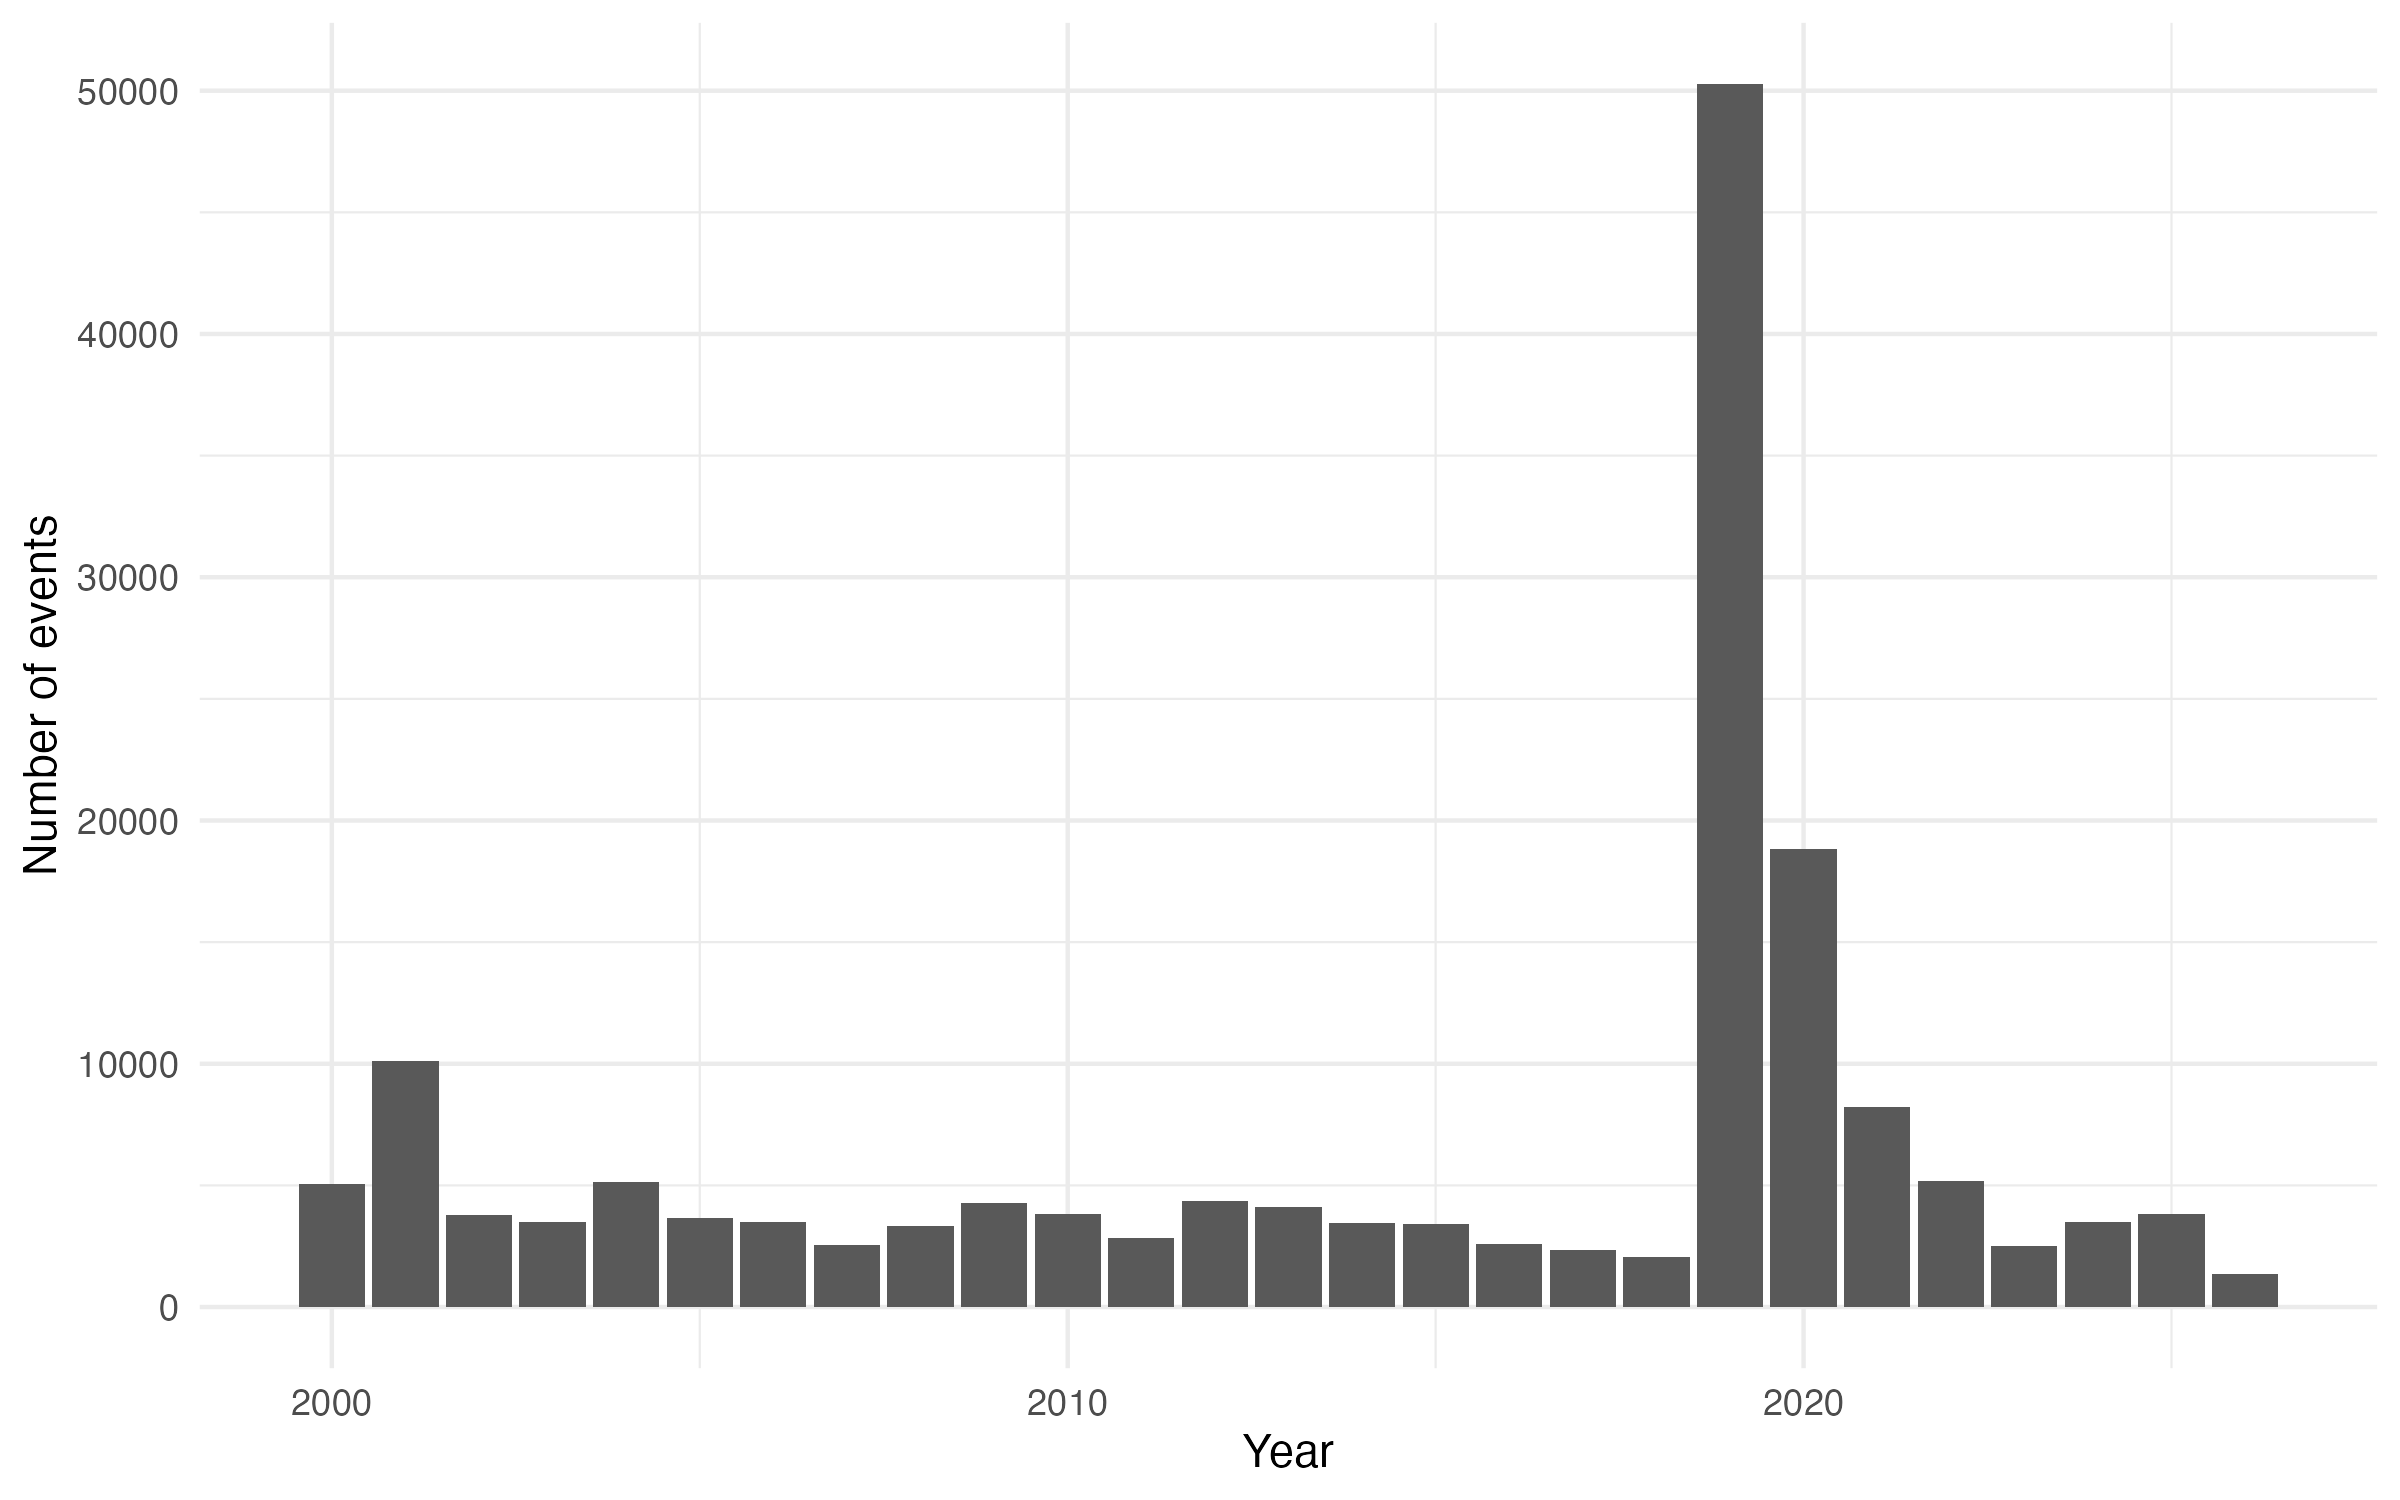
\includegraphics[width=0.88\textwidth]{annual_event_counts.png}
  \caption{Annual event counts in the pre-threshold catalogue. The pronounced
  increase in 2019 motivates the period-specific completeness and
  declustering summaries.}
  \label{fig:eda_temporal}
\end{figure}

The catalogue-wide MBS-WW estimate was approximately $M_c=1.7$. The
period-specific estimates were materially different: $M_c=3.3$ for 2019 and
$M_c=1.9$ for all other years. At $M_c=1.7$, the GFT values were 92.6\% for
2019 and 90.8\% for non-2019 events, meeting the secondary 90\% criterion but
not the 95\% criterion. Rolling 1,000-event windows showed that the largest
MBS-WW estimates were concentrated around 2019 rather than being uniformly
high across the observation period (Figure~\ref{fig:rolling_mc}).

\begin{figure}[htbp]
  \centering
  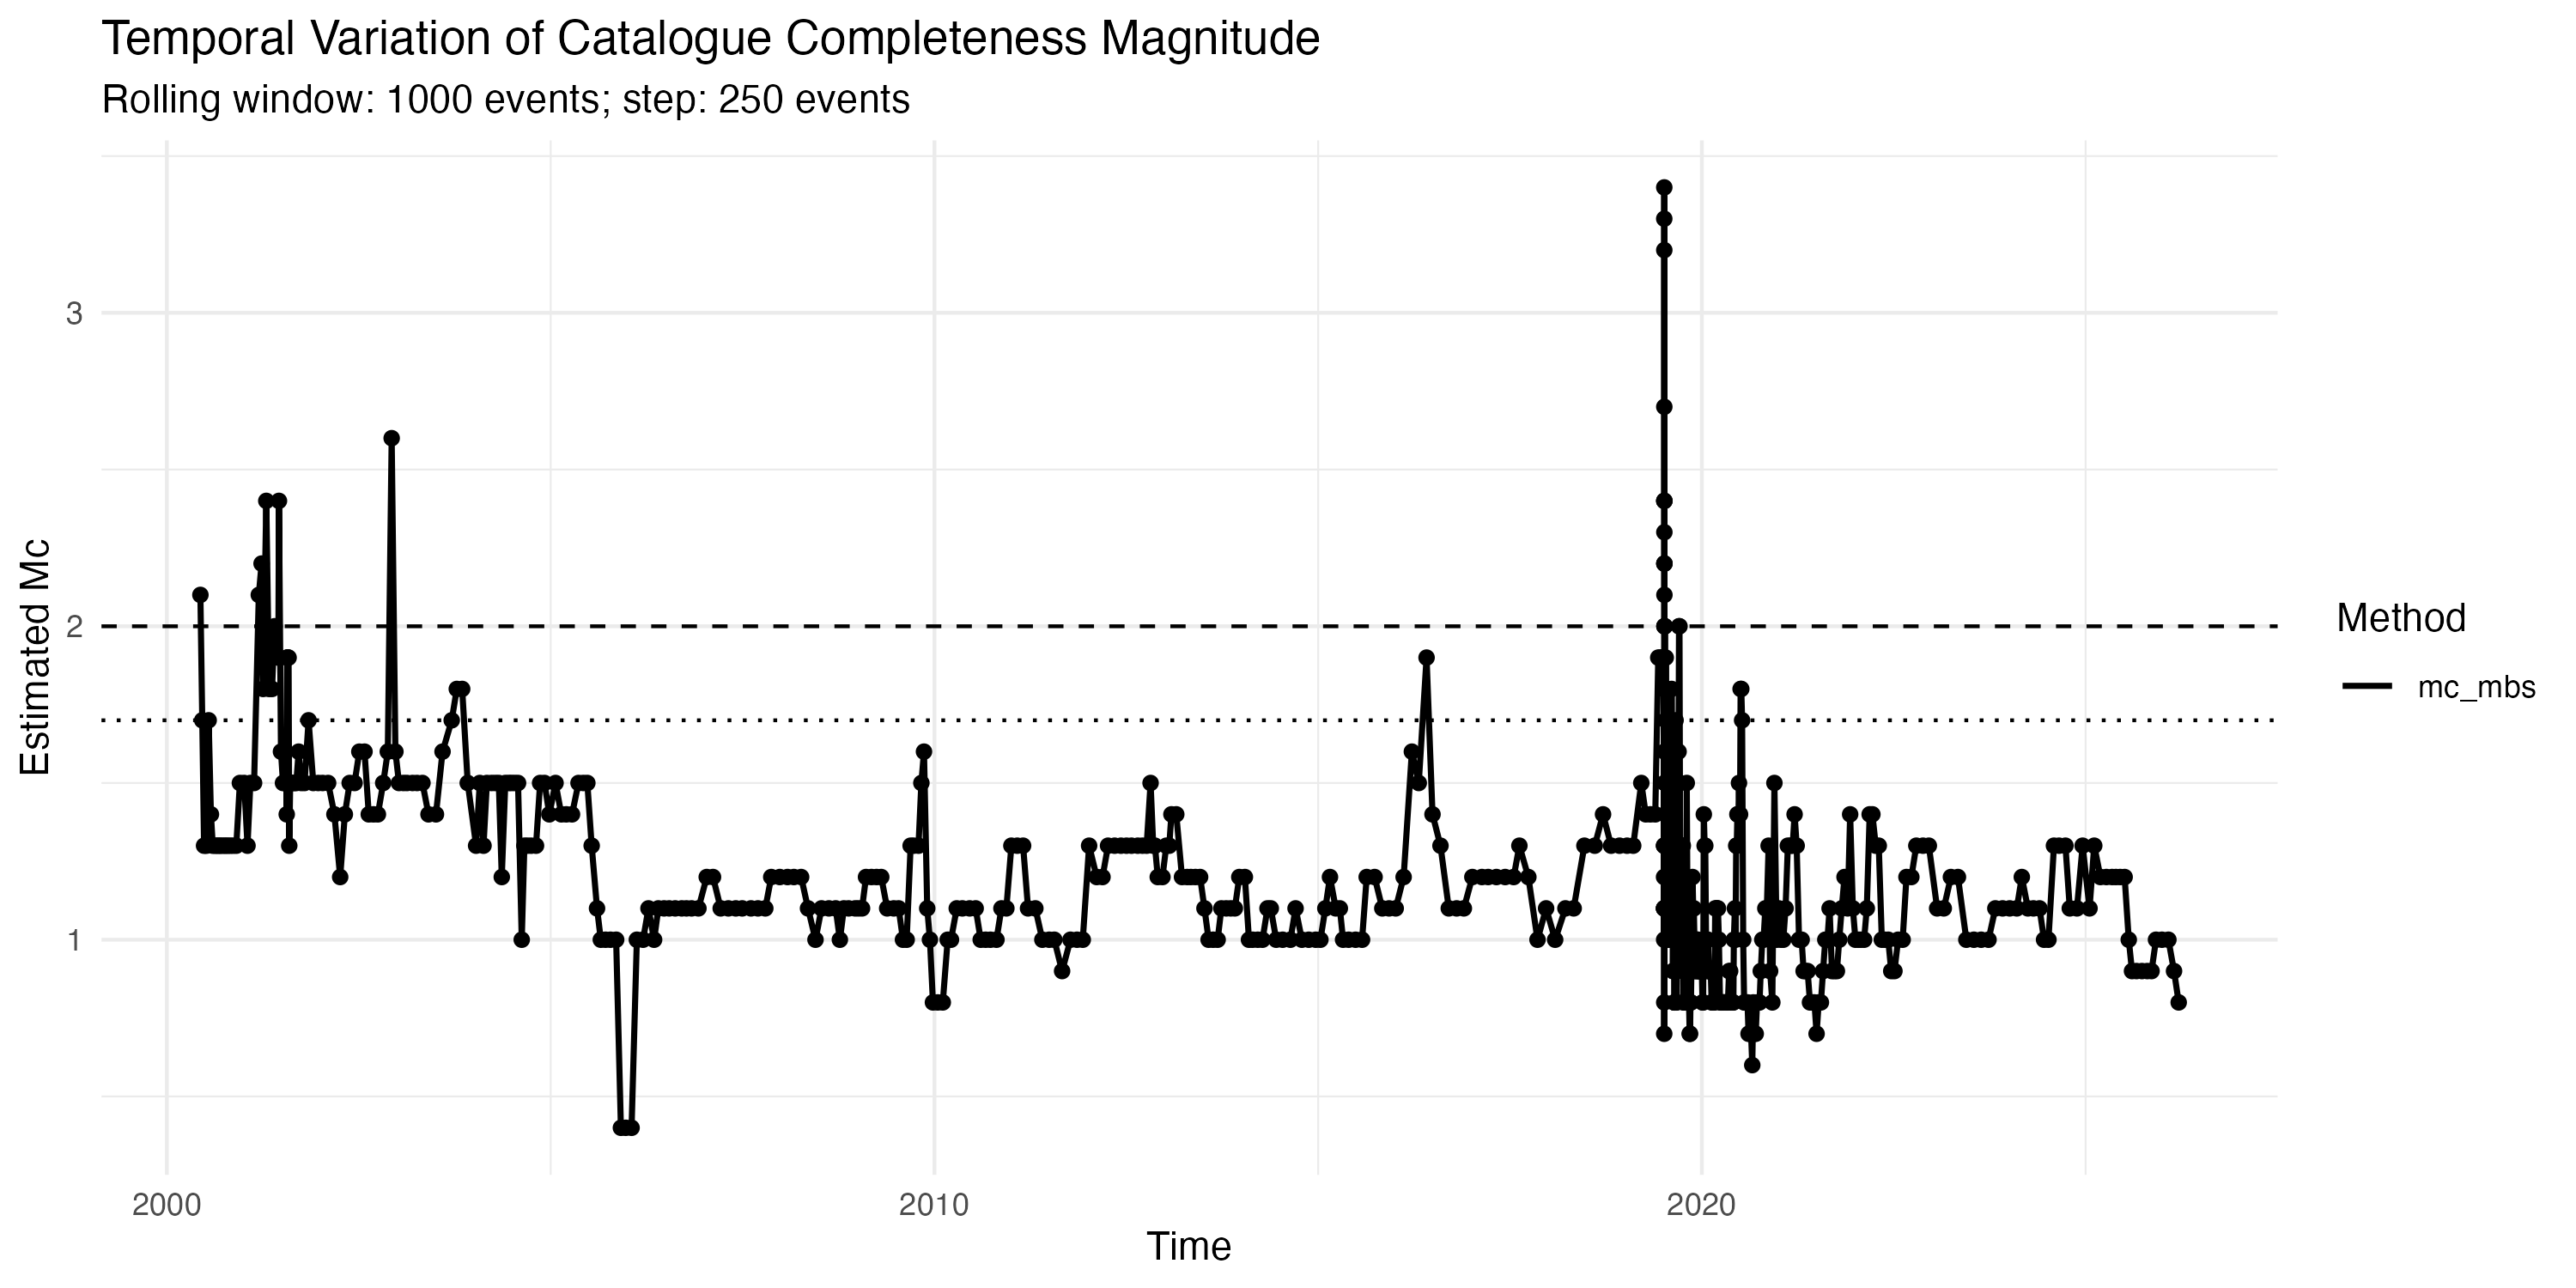
\includegraphics[width=0.88\textwidth]{Temporal_Mc_Rolling_Window.png}
  \caption{MBS-WW magnitude-completeness estimates in rolling windows of
  1,000 events in the pre-threshold catalogue.}
  \label{fig:rolling_mc}
\end{figure}

A common operational threshold of $M_c=2.0$ was adopted to preserve a single
catalogue for the controlled comparison while being more cautious than the
catalogue-wide estimate. This threshold retained 15,207 events, of which
6,865 (45.1\%) occurred in 2019. It remained below the separate 2019 estimate
of 3.3 and therefore does not establish complete detection throughout that
high-activity year.

\subsection{Evidence for triggering and a time-varying background}
\label{sec:results_nonstationarity}

The homogeneous Poisson model had log-likelihood $-8,046.72$, whereas the
stationary ETAS model had log-likelihood $27,577.37$ (Table~\ref{tab:model_comparison}).
The corresponding AIC difference was 71,240.18 and the BIC difference was
71,209.66 in favour of stationary ETAS, showing that a constant-rate process
without triggering was a poor relative description of these data.

Allowing the diagnostic ETAS background rate to vary across approximately
five-year intervals further increased the log-likelihood to $27,673.39$.
Relative to stationary ETAS, AIC decreased by 182.03 and BIC by 143.89 despite
the five additional parameters. This supported the use of a time-varying
background in the main model, although it did not by itself establish absolute
model adequacy.

\begin{table}[htbp]
\centering
\caption{Model comparisons used to motivate triggering and temporal variation
in the background rate. Lower AIC and BIC indicate better relative fit.}
\label{tab:model_comparison}
\begin{tabular}{lrrrr}
\toprule
Model & Log-likelihood & $k$ & AIC & BIC \\
\midrule
Homogeneous Poisson & $-8046.72$ & 1 & $16095.43$ & $16103.06$ \\
Stationary ETAS & $27577.37$ & 5 & $-55144.75$ & $-55106.60$ \\
Diagnostic non-stationary ETAS & $27673.39$ & 10 & $-55326.78$ & $-55250.49$ \\
\bottomrule
\end{tabular}
\end{table}

\subsection{Declustering-induced classification differences}
\label{sec:results_declustering}

The three methods assigned different background-like fractions to the same
15,207 events (Table~\ref{tab:declustering_summary}). Gardner--Knopoff
classified 2,599 events (17.1\%) as background-like, compared with 4,573
(30.1\%) for nearest-neighbour and 3,847 (25.3\%) for Reasenberg-style. Thus,
the largest difference, between Gardner--Knopoff and nearest-neighbour, was
13.0 percentage points. Across all three methods, 2,514 events (16.5\%) did
not receive a unanimous classification.

\begin{table}[htbp]
\centering
\caption{Event classifications from the three declustering methods using the
common $M\geq2.0$ catalogue.}
\label{tab:declustering_summary}
\begin{tabular}{lrrr}
\toprule
Method & Background-like & Clustered & Background-like (\%) \\
\midrule
Gardner--Knopoff & 2599 & 12608 & 17.1 \\
Nearest-neighbour & 4573 & 10634 & 30.1 \\
Reasenberg-style & 3847 & 11360 & 25.3 \\
\bottomrule
\end{tabular}
\end{table}

Pairwise raw agreement ranged from 0.852 to 0.915
(Table~\ref{tab:declustering_agreement}). Agreement on the background-like
class was weaker: Jaccard similarity ranged from 0.523 to 0.734. The
nearest-neighbour and Reasenberg-style classifications were closest
($\kappa=0.789$, Jaccard $=0.734$), while Gardner--Knopoff and
nearest-neighbour were furthest apart ($\kappa=0.600$, Jaccard $=0.523$).

\begin{table}[htbp]
\centering
\caption{Pairwise event-level agreement. Jaccard similarity is calculated for
the background-like sets.}
\label{tab:declustering_agreement}
\begin{tabular}{lrrr}
\toprule
Comparison & Raw agreement & Jaccard & Cohen's $\kappa$ \\
\midrule
GK vs NN & 0.852 & 0.523 & 0.600 \\
GK vs Reasenberg & 0.902 & 0.624 & 0.709 \\
NN vs Reasenberg & 0.915 & 0.734 & 0.789 \\
\bottomrule
\end{tabular}
\end{table}

Class imbalance was particularly strong in 2019. The background-like
fractions were 0.9\% for Gardner--Knopoff, 3.6\% for nearest-neighbour, and
2.0\% for Reasenberg-style. Pairwise raw agreement consequently exceeded
0.972 because almost all events were labelled clustered. In contrast, the
2019 Jaccard similarities were 0.235 for GK--NN, 0.420 for GK--Reasenberg,
and 0.512 for NN--Reasenberg, with corresponding $\kappa$ values of 0.371,
0.586, and 0.668. The high raw agreement therefore reflected agreement on the
dominant clustered class, not interchangeable identification of the small
background-like subset.

\subsection{Declustering-derived starting backgrounds}
\label{sec:results_initialisation}

The classification differences propagated into the raw monthly background
rates. Over the full period, the GK--NN monthly comparison had MAE $0.209$
events/day, RMSE $0.324$ events/day, and correlation $0.490$. GK--Reasenberg
had MAE $0.133$, RMSE $0.180$, and correlation $0.687$, while NN--Reasenberg
had MAE $0.091$, RMSE $0.185$, and correlation $0.841$. During 2019 the
GK--NN differences increased to MAE $0.502$ and RMSE $0.632$ events/day, and
the correlation was $-0.167$.

Table~\ref{tab:initial_background_metrics} reports the smooth functions that
were actually supplied to the ETAS optimiser, evaluated on the common daily
grid after applying the pseudo-count, exposure adjustment, spline projection,
and ridge stabilisation. The largest difference remained GK--NN, with MAE
$0.203$ and RMSE $0.295$ events/day. Its correlation decreased to 0.302 after
spline projection, indicating that the two starts differed in temporal shape
as well as level. NN--Reasenberg had the smallest MAE ($0.076$) and the
highest correlation (0.931). These values establish that the main experiment
did not begin from nearly identical background functions.

\begin{table}[htbp]
\centering
\caption{Pairwise differences between the smooth background functions used as
ETAS starting values, evaluated on the common daily grid. MAE and RMSE are in
events/day; correlation is dimensionless.}
\label{tab:initial_background_metrics}
\begin{tabular}{lrrr}
\toprule
Comparison & MAE & RMSE & Correlation \\
\midrule
GK vs NN & 0.203052 & 0.294838 & 0.302010 \\
GK vs Reasenberg & 0.129409 & 0.155881 & 0.503749 \\
NN vs Reasenberg & 0.076162 & 0.158183 & 0.930644 \\
\bottomrule
\end{tabular}
\end{table}

\subsection{Sensitivity of fitted ETAS inference to initialisation}
\label{sec:results_etas}

All three main fits returned convergence code 0. The triggering estimates and
unpenalised log-likelihoods were very similar
(Table~\ref{tab:etas_parameters}). The largest pairwise ranges were
$2.09\times10^{-5}$ for $K$, $5.53\times10^{-4}$ for $\alpha$,
$2.50\times10^{-5}$ days for $c$, and $3.98\times10^{-4}$ for $p$. The
unpenalised log-likelihoods differed by 0.121 across the three fits. The
penalised objectives were $-27765.576$, $-27765.584$, and $-27765.582$ for
GK, NN, and Reasenberg-style starts, respectively, a total range below 0.009.
These numerical differences do not constitute a formal equivalence test, but
they show low fitted-parameter sensitivity across the three starts examined.

\begin{table}[htbp]
\centering
\caption{Non-stationary ETAS fits from the three declustering-derived
background starts. Log-likelihood is unpenalised; all convergence codes were
zero.}
\label{tab:etas_parameters}
\begin{tabular}{lrrrrr}
\toprule
Initialisation & Log-likelihood & $K$ & $\alpha$ & $c$ & $p$ \\
\midrule
Gardner--Knopoff & 27767.432 & 0.020154 & 1.588437 & 0.009616 & 1.122273 \\
Nearest-neighbour & 27767.466 & 0.020157 & 1.588518 & 0.009610 & 1.122048 \\
Reasenberg-style & 27767.553 & 0.020175 & 1.587965 & 0.009591 & 1.121875 \\
\bottomrule
\end{tabular}
\end{table}

The final fitted background functions were also nearly coincident. Pairwise
final correlations exceeded 0.999991 and final MAEs ranged from 0.000779 to
0.001063 events/day. Comparing initial and final functions on the same daily
grid gave MAE ratios of 0.00384, 0.00822, and 0.01174
(Table~\ref{tab:propagation}). Thus, approximately 0.38\%--1.17\% of the
initial MAE remained, corresponding to 98.83\%--99.62\% attenuation. The
RMSE ratios were 0.00322--0.00896, corresponding to 99.10\%--99.68\%
attenuation. The same-grid correction therefore leaves the substantive
conclusion unchanged while replacing the earlier comparison of different
time grids.

\begin{table}[htbp]
\centering
\caption{Propagation of differences between initial and final background-rate
functions on a common daily grid. MAE and RMSE are in events/day.}
\label{tab:propagation}
\resizebox{\textwidth}{!}{%
\begin{tabular}{lrrrrrrr}
\toprule
Comparison & Initial MAE & Final MAE & MAE ratio & Initial RMSE & Final RMSE & RMSE ratio & Final $r$ \\
\midrule
GK vs NN & 0.203052 & 0.000779 & 0.003835 & 0.294838 & 0.000951 & 0.003224 & 0.999991 \\
GK vs Reasenberg & 0.129409 & 0.001063 & 0.008216 & 0.155881 & 0.001396 & 0.008957 & 0.999993 \\
NN vs Reasenberg & 0.076162 & 0.000894 & 0.011744 & 0.158183 & 0.001177 & 0.007442 & 0.999993 \\
\bottomrule
\end{tabular}}
\end{table}

Taken together, the main experiment shows substantial differences in event
labels and starting background functions, followed by only very small
differences in the fitted ETAS parameters and background function under the
baseline model and catalogue.

\subsection{Model-specification robustness}
\label{sec:results_robustness}

All three alternative specifications returned convergence code 0
(Table~\ref{tab:robustness}). Relative to the eight-degree-of-freedom
baseline, six degrees of freedom reduced the log-likelihood by 15.20 and ten
degrees of freedom increased it by 2.98. Extending the cutoff to 7,300 days
changed the log-likelihood by $-0.44$. Across the alternatives, the largest
percentage changes were 0.41\% for $K$, 0.12\% for $\alpha$, 3.38\% for
$c$, and 0.42\% for $p$.

The final background was most affected by reducing spline flexibility:
relative to baseline, the six-degree-of-freedom curve had MAE $0.0280$
events/day, RMSE $0.0410$, and correlation 0.9825. The ten-degree-of-freedom
curve had MAE $0.0128$, RMSE $0.0179$, and correlation 0.9966. Extending the
cutoff had the smallest effect (MAE $0.00536$, RMSE $0.00671$, correlation
0.99979). These results show some expected sensitivity of the background
curve to its flexibility but no large change in the triggering estimates.
They do not establish initialisation robustness under the alternative
specifications because those models were fitted only from the
nearest-neighbour start.

\begin{table}[htbp]
\centering
\caption{Limited ETAS specification robustness with the nearest-neighbour
initialisation fixed. Background MAE and correlation compare each fitted
background function with the baseline.}
\label{tab:robustness}
\resizebox{\textwidth}{!}{%
\begin{tabular}{lrrrrrrrr}
\toprule
Specification & Log-likelihood & $K$ & $\alpha$ & $c$ & $p$ & Background MAE & Background RMSE & Background $r$ \\
\midrule
Baseline (df 8; 3650 d) & 27767.466 & 0.020157 & 1.588518 & 0.009610 & 1.122048 & -- & -- & -- \\
df 6; 3650 d & 27752.268 & 0.020202 & 1.587419 & 0.009935 & 1.126762 & 0.027989 & 0.040999 & 0.982543 \\
df 10; 3650 d & 27770.450 & 0.020239 & 1.586574 & 0.009495 & 1.120410 & 0.012818 & 0.017872 & 0.996613 \\
df 8; 7300 d & 27767.029 & 0.020155 & 1.588306 & 0.009673 & 1.123139 & 0.005357 & 0.006712 & 0.999792 \\
\bottomrule
\end{tabular}}
\end{table}

\section{Discussion}
\label{sec:discussion}

The three declustering schemes produced materially different event labels and
different background-rate starting functions, but those differences were
almost completely attenuated when the same baseline non-stationary ETAS model
was fitted to the same catalogue. All three fits converged to very similar
triggering parameters, unpenalised log-likelihoods, penalised objectives, and
fitted background functions. On a common daily grid, only 0.38\%--1.17\% of
the initial pairwise MAE remained. The evidence therefore indicates that, for
this catalogue and model specification, the fitted ETAS inference was highly
robust to the three declustering-derived initialisations. Although
demonstrated using a Southern California catalogue, this finding has a
broader methodological implication: when declustering is used solely to
initialise a background component that is subsequently updated during
penalised likelihood optimisation, substantial differences between the
starting background estimates may be largely attenuated. Whether this
robustness extends to other catalogues, declustering algorithms, and model
specifications requires further investigation; the result should not be
interpreted as evidence that declustering is generally unimportant.

The disagreement among the three methods is plausible because they
operationalise earthquake clustering differently: Gardner--Knopoff applies
magnitude-dependent space--time windows, the nearest-neighbour method uses
data-derived space--time--magnitude links, and the Reasenberg-style method
constructs interacting event groups that can expand or merge. Comparative
studies have similarly shown that declustering methods can retain different
numbers and types of events and that both algorithm and parameter choices can
affect the resulting catalogue summaries
\citep{perry2024comparative,mizrahi2021effect}.

In the present analysis, the proportion of events classified as
background-like ranged from 17.1\% for Gardner--Knopoff to 30.1\% for the
nearest-neighbour method, a difference of 13.0 percentage points. Moreover,
16.5\% of events did not receive the same classification from all three
methods. These differences would be important if the classifications were
used to remove events or define the final background catalogue. Here,
however, they were used only to construct alternative starting
background-rate functions. All events remained in the ETAS likelihood, and
the background function was re-estimated during optimisation. This helps
explain why substantial disagreement in the initial classifications did not
translate into material differences in the final ETAS solution.

The 2019 results show why the overall percentage of matching classifications
was not sufficient to describe agreement between the methods. Because almost
all events were classified as clustered, the methods agreed on more than
97\% of all events. However, they agreed much less on which events were
background-like. For example, among the events classified as background-like
by either Gardner--Knopoff or the nearest-neighbour method, only 23.5\% were
classified as background-like by both methods, as indicated by their Jaccard
index of 0.235. The high overall agreement therefore concealed important
disagreement about the relatively small set of events used to construct the
initial background rate. The largest differences between the monthly
starting rates also occurred in 2019. This connects the unusually high
earthquake activity identified in the exploratory analysis with the observed
differences in model initialisation.

Here, attenuation refers to the reduction in the differences between the
three starting background-rate functions after the ETAS model was fitted. On
the common daily grid, the pairwise MAEs between the final background-rate
functions were only 0.38--1.17\% of the corresponding MAEs between the
starting functions, equivalent to reductions of 98.83--99.62\%. This pattern
can be understood from the experimental design. Declustering supplied only
the starting background functions; it did not constrain the fitted
background to remain close to them. After initialisation, every fit
re-estimated the background and triggering parameters by optimising the same
penalised likelihood using the same events, spline basis, penalty, parameter
bounds, and triggering-parameter starts. The nearly identical final
log-likelihoods, parameters, and background-rate functions therefore show
that the three declustering-derived starts led the optimiser to essentially
the same numerical solution.

This result does not establish that the penalised likelihood has a unique
global optimum. Direct likelihood estimation of ETAS models can be
computationally demanding and unstable, particularly when the likelihood
surface is flat or contains multiple local optima, and its performance may
depend on the starting values \citep{veen2008estimation,lombardi2015simulated}.
Neutral and randomly perturbed multi-start fits were available as optional
code in the present analysis but were not executed. The observed convergence
of the three scientifically motivated starts therefore demonstrates
robustness to those starts, rather than general independence from starting
values or proof of a global optimum.

The model-screening results also clarify the role of the non-stationary
background. Stationary ETAS was strongly preferred to a homogeneous Poisson
process, and the diagnostic piecewise-background model improved both AIC and
BIC relative to stationary ETAS. This supports separating temporal changes in
background activity from earthquake-to-earthquake triggering. Previous
non-stationary ETAS work has represented a time-varying background with
splines and estimated it jointly with triggering parameters under a roughness
penalty \citep{kattamanchi2017nonstationary}. The present study contributes a
different sensitivity question: whether three scientifically motivated
background starts derived from alternative declustering rules persist after
joint optimisation.

A principal strength of the study is its controlled comparison. Only the
declustering-derived starting background function changed between the three
main fits; the catalogue events included in the likelihood and all other
baseline modelling choices were held fixed. This design made it possible to
isolate whether the choice of starting background materially altered the
fitted ETAS inference. Examining the classifications, the background
functions constructed from them, and the final model estimates also showed
where the differences arose and whether they persisted after optimisation.
Agreement was evaluated using Jaccard similarity and $\kappa$ as well as the
overall percentage agreement, preventing the dominant clustered category
from concealing disagreement about the less common background-like events.
Pairwise errors calculated on the same daily grid then measured how much of
the initial difference remained in the fitted background functions. The
limited specification checks provided additional evidence that the
triggering estimates were not strongly affected by moderate changes in
spline flexibility or triggering-history length, while the observed changes
in the background curve also show that this reassurance is not equivalent to
complete model-specification robustness.

The findings nevertheless have important limitations. First, the study used
one regional catalogue, so external validity across tectonic settings,
network histories, and magnitude ranges is unknown. Second, the common
$M_c=2.0$ threshold was below the 2019 MBS-WW estimate of 3.3. Residual
incompleteness during the most active sequence could alter nearest-neighbour
relationships, window membership, and the division of ETAS intensity into
background and triggering components. A time-varying completeness model or a
focused analysis above a higher 2019 threshold could address this issue, but
neither was part of the present results.

Third, each declustering method used one baseline parameterisation. The
experiment therefore measures sensitivity to three implemented starting
functions, not uncertainty over all plausible declustering parameter values.
The nearest-neighbour classification was deterministic and simpler than the
stochastic, spatially adaptive procedure in \citet{zaliapin2020declustering},
and the Reasenberg-style implementation was not an exact reproduction of
\texttt{CLUSTER2000}. Fourth, the ETAS model was temporal rather than
spatio-temporal. Spatial heterogeneity affected declustering but was not
modelled in the ETAS background or triggering kernel.

Fifth, the baseline spline degrees of freedom, fixed penalty, parameter
bounds, and 3,650-day cutoff are modelling choices. The robustness analysis
varied only degrees of freedom and the cutoff, and only from the
nearest-neighbour start; it did not examine the penalty or the full
initialisation-by-specification combination. The analysis also ignored
triggering before the catalogue boundary. Sixth, convergence code 0 and close
objectives do not alone establish a global optimum. The absence of neutral or
jittered extra starts limits the strength of claims about generic optimiser
robustness.

Finally, uncertainty summaries were descriptive. No standard errors,
confidence intervals, bootstrap analysis, or formal equivalence margins were
computed for differences among fitted parameters or curves. Point-process
residual diagnostics, such as a time-rescaling assessment, were also not
reported, so relative AIC/BIC improvement should not be interpreted as proof
of absolute fit. The study did not evaluate forecasts; similarity of fitted
parameters cannot be extended to predictive equivalence.

For practice, the results suggest that when reasonable declustering outputs
are used only to initialise a background function that is re-estimated during
penalised non-stationary ETAS fitting, the final inference may be much less
sensitive than the initial event classifications imply. Analysts should
nevertheless record the declustering method, inspect agreement on the less
common background-like classification, use multiple optimisation starts, and
compare final objectives and fitted curves. Differences between declustering
methods may matter more when the resulting catalogues are analysed as
different datasets, when the fitted background is constrained towards its
initial estimate, or when the likelihood has more pronounced local modes.

In plain terms, the three declustering methods disagreed about which
earthquakes looked like background activity, especially during the crowded
2019 sequence. Yet, once those alternatives were used only as starting points
for the same statistical model, the fitted model arrived at almost the same
answer. For this catalogue and baseline specification, the ETAS inference was
robust to the three starting backgrounds, while the disagreement in the
original event labels remains real and should not be ignored.
